%!TEX root = ../main.tex
%%%%%%%%%%%%%%%%%%%%%%%%%%%%%%%%%%
% Links:
%
% Difficulty:
% Companies: 
%%%%%%%%%%%%%%%%%%%%%%%%%%%%%%%%%%


%\begin{figure}
%   \centering
%   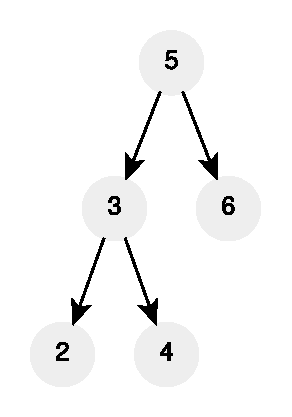
\includegraphics[width=\textwidth]{sources/kth_smallest_in_sorted_matrix/images/example1}
%   \caption[Sample short cpation]{Sample Caption}.
%   \label{fig:kth_smallest_in_sorted_matrix:example1}
%\end{figure}

\chapter{$k^{th}$ smallest element in a sorted matrix}
\label{ch:kth_smallest_in_sorted_matrix}
\section*{Introduction}
\begin{wraptable}{r}{4.5cm}
    \centering
    \begin{framed}  
    \begin{tabular}{|c|c|c|}
    \hline
    1  & 5  & 9  \\ \hline
    10 & 12 & 13 \\ \hline
    12 & 13 & 15 \\ \hline
\end{tabular}%
\caption{Tabular representation of Example \ref{example:kth_smallest_in_sorted_matrix:example1}}
\label{tab:kth_smallest_in_sorted_matrix:example1}
\end{framed}
\end{wraptable} 

One of the most common tool in computer science and engineering in general are rectangular grids of number also known as matrices\footnote{Matrices however are not stored in memory as grids. Computer memory is linear (think of it as an array) and therefore matrices must be mapped into it in some way. Turns out there is not only a single way of performing such a mapping, with the most common ones being \textit{row-major} and \textit{column-major}. The row-major stores each rows one after the other contiguously in memory  while column-major does the same but with columns. The matrix in Example \ref{example:kth_smallest_in_sorted_matrix:exercice1} would be stored as $\{\underbrace{1,5,9}_{\text{row 0}},\underbrace{10,12,13}_{\text{row 1}},\underbrace{12,13,15}_{\text{row 2}}\}$ in a row-major mapping and as $\{\underbrace{1,10,12}_{\text{col 0}},\underbrace{5,12,13}_{\text{col 1}},\underbrace{9,13,15}_{\text{col 2}}\}$as column-major.}. The data they  contain can represent many things, from mathematical set of linear equations to algorithm for compression of images and videos or graphs.

In this chapter, we are not going to worry about all of those fancy applications of matrices, and instead, we will focus on a much simpler problem on a class of matrices of integers with the property of having rows and columns sorted. The task we need to perform on such a matrix is one that is easily explained: we have to find the $k^{th}$ smallest number among \textbf{all} values in the matrix.
This is one such problem for which we will be able to find a working solution straight away, but coming up with a more efficient time and space solution is way more complicated. 
On top of that, the naive solution differs conceptually quite a bit from the faster ones and that further complicates things, especially during an interview. Most of us, once the naive solution is found, are naturally driven towards optimizing it rather than trying to think about a radically different way to approach the problem which, as we will see below, is key to finding solutions with better asymptotic complexity.



\section{Problem statement}
\begin{exercise}
\label{example:kth_smallest_in_sorted_matrix:exercice1}
Write a function that, given an square matrix $M$ of size $n$  where each of individual row and column is sorted in ascending order and an integer $1 \leq k \leq n^2$
returns the $k^{th}$ smallest element in $M$.


You can assume the elements of $M$ to be always in the range $[0,n^2]$.

    %example1
    \begin{example}
        \label{example:kth_smallest_in_sorted_matrix:example1}
        \hfill \\
        Given $M=\{\{1,5,9\},\{10,12,13\},\{12,13,15\}\}$ (as shown in Table \ref{tab:kth_smallest_in_sorted_matrix:example1}) and $k=8$ the function returns $13$.
    \end{example}
\end{exercise}




\section{Clarification Questions}

\begin{QandA}
    \item Can we assume the input to be always valid i.e. having rows and column sorted?
    \begin{answered}
        \textit{Yes, there is no need to perform any input validation whatsoever.}
    \end{answered}
    
    \item Can $M$ contains duplicates?
    \begin{answered}
        \textit{Yes.}
    \end{answered}
    
\end{QandA}

\subsection{Brute-force}
\label{kth_smallest_in_sorted_matrix:sec:bruteforce}
A quick solution to this problem would be to copy into a vector \textbf{all} elements of $M$. If can sort this vector we will have the answer at location  $k-1$. 
This solution, implemented in Listing \ref{list:kth_smallest_in_sorted_matrix:bruteforce}, is simple, easy to explain and implement, and most importantly is correct. 

\lstinputlisting[language=c++, caption={Naive brute-force solution.},label=list:kth_smallest_in_sorted_matrix:bruteforce]{sources/kth_smallest_in_sorted_matrix/kth_smallest_in_sorted_matrix_solution1.cpp}

The code works by copying every single row of $M$ into a temporary array \inline{M_linear} that we then proceed to sort. We can notice how in reality \inline{M_linear} is not really sorted fully, but only partially by using \inline{std::partial_sort}\cite{cit::std::partialsort} (see Section \ref{sec:find_k_closest_in_array:sorting} for another problem where we used this type of sorting) which is called in such a way that the smallest $k$ elements of $M$ are moved to the front of \inline{M_linear} and are properly sorted leaving the rest of \inline{M_linear} unsorted. That is OK because we do not really care about anything but the $k^{th}$ smallest elements.
We use \inline{std::partial_sort} as this way the overall complexity of this approach is dependent on $k$ instead of the total number of elements in $M$. When $k << |M|$ this can result in measurable performance improvements. However, this does not really change the overall time final asymptotical complexity as $K$ can be as big as $|M|$.
The time and space complexities are therefore $O(nm\times log(nm)$) and $O(nm)$, respectively, where $nm$ is the number of elements in $M$.

\subsection{Brute-force improved}
\label{kth_smallest_in_sorted_matrix:sec:bruteforce_constant_space}
In Section \ref{kth_smallest_in_sorted_matrix:sec:bruteforce} we solved the problem by pure brute-force and we did not take advantage of the fact that rows and columns are sorted to begin with. 
A possible way we can use this fact to our advantage is to use two pointers \inline{rightPtr}, and \inline{downPtr} to navigate rows and columns, respectively. \inline{rightPtr} will always move to the right (thus inspecting rows) and \inline{downPtr} will go downwards to take care of columns. 
Our claim is that we can move these two pointers one at a time by advancing the one pointing to the smallest element, and visit $M$ respecting the total order of its elements.

First of all, we should notice that the smallest element will always be at the top-left corner (location $(0,0)$ in $M$).
If we initialize them so that \inline{rightPtr=(0,1)} and \inline{downPtr=(1,0)}, then we know that the \nth{1} smallest element is pointed by \inline{downPtr} and the \nth{2} smallest is the smallest between  \inline{rightPtr} and \inline{downPtr}. Whenever a pointer points to the next smallest element, we move it in its prefeered direction (\inline{rightPtr} to the right and \inline{downPtr} downwards). Of course when a pointer reached the limit of the matrix we make sure to move it either to the next row or column and we make sure to make it start so that we avoid cells that have been already visited. Given \inline{downPtr = (p,q)}, when we need to wrap around \inline{rightPtr = (x,y)} we can move it to \inline{(x+1,q+1)} i.e. to the next row, but avoiding looking at any column that have been already looked by \inline{downPtr}. Similarly, when we need to wrap around \inline{downPtr = (p,q)} we make sure to avoid rows already taken into account by \inline{rightPtr} by setting it to \inline{rightPtr = (x+1,q+1)}. 

If we continue to move these pointers then, after we have moved them $k^{th}$ times we know for sure that one of the two pointers points to the final answer and in particular, the smallest of the two is the value we need.
Figure \ref{fig:kth_smallest_in_sorted_matrix:visitall} shows how this work using the instance in Example \ref{example:kth_smallest_in_sorted_matrix:example1}.

\begin{figure}
    \centering
    \begin{subfigure}[t]{0.32\textwidth}
        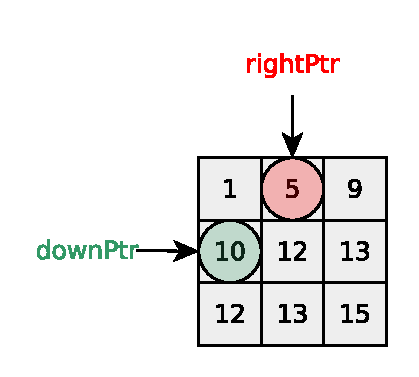
\includegraphics[width=1\linewidth]{sources/kth_smallest_in_sorted_matrix/images/visit1}
        \caption{}
        \label{fig:kth_smallest_in_sorted_matrix:visit1}
     \end{subfigure}
    \hfill
    \begin{subfigure}[t]{0.32\textwidth}
        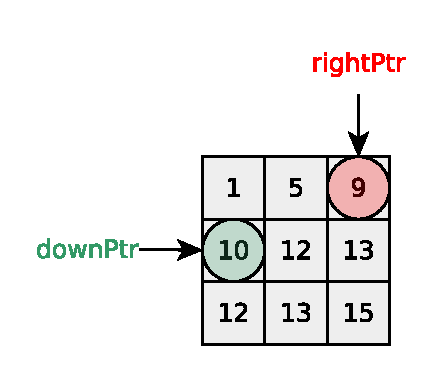
\includegraphics[width=1\linewidth]{sources/kth_smallest_in_sorted_matrix/images/visit2}
        \caption{}
        \label{fig:kth_smallest_in_sorted_matrix:visit2}
     \end{subfigure}
     \hfill
    \begin{subfigure}[t]{0.32\textwidth}
        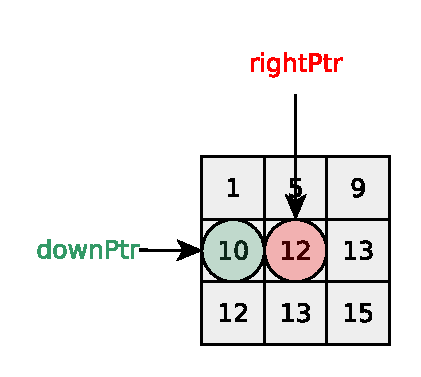
\includegraphics[width=1\linewidth]{sources/kth_smallest_in_sorted_matrix/images/visit3}
        \caption{}
        \label{fig:kth_smallest_in_sorted_matrix:visit3}
     \end{subfigure}
     \hfill
    \begin{subfigure}[t]{0.32\textwidth}
        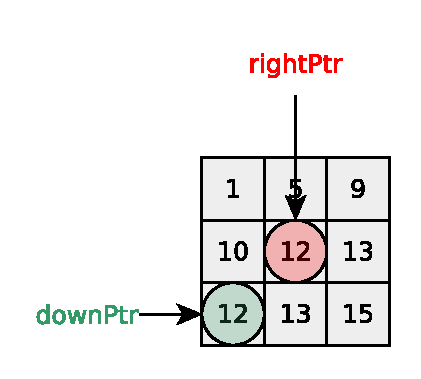
\includegraphics[width=1\linewidth]{sources/kth_smallest_in_sorted_matrix/images/visit4}
        \caption{}
        \label{fig:kth_smallest_in_sorted_matrix:visit4}
    \end{subfigure}
    \hfill
    \begin{subfigure}[t]{0.32\textwidth}
        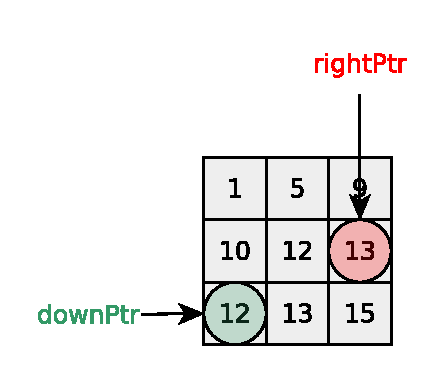
\includegraphics[width=1\linewidth]{sources/kth_smallest_in_sorted_matrix/images/visit5}
        \caption{}
        \label{fig:kth_smallest_in_sorted_matrix:visit5}
    \end{subfigure}
    \hfill
    \begin{subfigure}[t]{0.32\textwidth}
        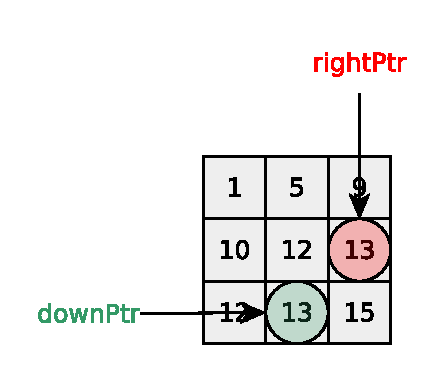
\includegraphics[width=1\linewidth]{sources/kth_smallest_in_sorted_matrix/images/visit6}
        \caption{}
        \label{fig:kth_smallest_in_sorted_matrix:visit6}
    \end{subfigure}
    \hfill
    \begin{subfigure}[t]{0.32\textwidth}
        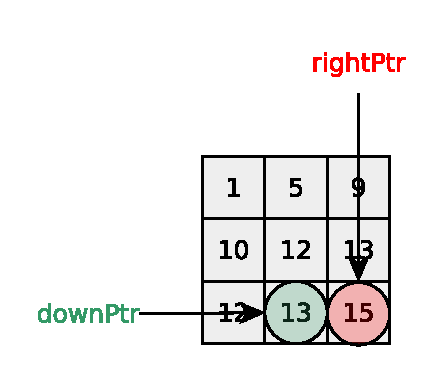
\includegraphics[width=1\linewidth]{sources/kth_smallest_in_sorted_matrix/images/visit7}
        \caption{}
        \label{fig:kth_smallest_in_sorted_matrix:visit7}
    \end{subfigure}
    
    

     \caption[Execution Listing \ref{list:kth_smallest_in_sorted_matrix:bruteforce_improved} on Example \ref{example:kth_smallest_in_sorted_matrix:example1}]{Execution Listing \ref{list:kth_smallest_in_sorted_matrix:bruteforce_improved} on Example \ref{example:kth_smallest_in_sorted_matrix:example1}. The pointers are initialized as shown in Figure \ref{fig:kth_smallest_in_sorted_matrix:visit1}. We then compare them and move \inline{rightPtr} to the right because it is the smallest among the two of them. Next we move it again as shown in Figure \ref{fig:kth_smallest_in_sorted_matrix:visit2} because the value it points to (i.e. $9$) is still smaller than the value pointed by \inline{downPtr}. We cannot move \inline{rightPtr} to the right as it would break the boundaries of the matrix and we therefore move it one row down but we carefully place it a column to the right of the column \inline{downPtr} is at (because \inline{downPtr} is taking care of that column). After that, in Figure \ref{fig:kth_smallest_in_sorted_matrix:visit4} we can see that  \inline{downPtr} is moved. At this point both pointers point to cells containing the same value. When a case like this happens we always choose to move \inline{rightPtr}. In Figure \ref{fig:kth_smallest_in_sorted_matrix:visit5} we see that \inline{downPtr} is moved again. Notice that, because we could not move it downwards, we moved it one column to the right and to a row below \inline{rightPtr}'s row. Up at this point we moved pointers $7$ times if we also consider cell $(0,0)$ that we skipped entirely. We only need to move it once more to be able to find the \nth{8} smallest. This last step is shown in Figure \ref{fig:kth_smallest_in_sorted_matrix:visit7} where \inline{rightPtr} is moved one row below and one column to the right of \inline{downPtr} column coordinate, finally landing in the last cell.}
      \label{fig:kth_smallest_in_sorted_matrix:visitall}
\end{figure}

Notice that there could be a case where it is impossible to move a pointer any further as it would go completely outside the boundaries of the matrix in both directions. When this happens, we should simply continue moving the other pointer and keep counting\footnote{We can think of this case as if the exhausted pointer would be always pointing to imaginary cells of infinite value.}.

An implementation of this idea is shown in Listing \ref{list:kth_smallest_in_sorted_matrix:bruteforce_improved}.

\lstinputlisting[language=c++, caption={Brute-force solution using constnat space.},label=list:kth_smallest_in_sorted_matrix:bruteforce_improved]{sources/kth_smallest_in_sorted_matrix/kth_smallest_in_sorted_matrix_solution2.cpp}

The main driver function, \inline{kth_smallest_in_sorted_matrix_brute_force_constant_space}, contains a bunch of loos with the first, being the main one. We can see there how \inline{downPtr} and \inline{rightPtr} are compared first and the smallest of the two is moved. In order to move them, two auxiliary functions are used: \inline{advanceDown} and \inline{advanceRight}. These functions make sure the pointers are moved properly so that if necessary the wrapping around described above is enforced. We can also notice that they return a boolean value which indicates whether the movement resulted in the pointer going outside the boundary of the matrix.
This boolean value is used to break out of the main loop in \inline{kth_smallest_in_sorted_matrix_brute_force_constant_space} and when this happens to decide which pointer needs to be moved further. If \inline{downPtr} went overboard the matrix then we continue moving \inline{rightPtr} and the other way round if \inline{rightPtr} went overboard. If we reach the end of the first main, then only the body of one of the two subsequent \inline{while} can be executed.

The time and space complexities of this approach are $O(nm)$ and $O(1)$, respectively, with $nm$ being the total number of cells in $M$.

\subsection{Binary Search}
\label{kth_smallest_in_sorted_matrix:sec:binarysearch}
So far, all the solutions we described are based on explicitly sorting the values of $M$. The first by literally sorting them and the second by performing a \quotes{in-order} visit (borrowing the terminology from binary search trees) of $M$. The issue with this approach is that we cannot get away with the fact we might need to end up visiting the entire matrix. We have a lower bound on the time complexity we can reach with any solution based on spelling out the values of $M$ in an ordered fashion: $O(nm)$.

But what if we try to guess what the value of the $k^{th}$ smallest could be and then check if that is indeed the right answer? The guessing part can be carried out using binary search and we know that we will not need more than $O(log(U))$ where $U$ is the difference between the smallest and largest element of $M$ (which are for sure places at cells $(0,0)$ and $(n-1.m-1)$).
However, guessing the number is only part of the story. Once we have a number, we must check that whether it can indeed be the answer or for sure it is not. 
We know that the $k^{th}$ element of $M$ is a value for which there are $k-1$ smaller or equal elements in $M$. We can use this definition to validate our guess. All we have to do is to visit $M$ and count the number that is lower or equal to our guess. However, doing it naively will actually cost us $O(nm)$ as we must look at every cell of $M$! This would result in a worse overall time complexity than the brute-force solution discusses above as we would perform $O(log(U))$ steps each costing $O(nm)$.

However, we can use the fact that rows and columns are sorted in order to speed up this coutning step.
The idea is that, if we want to count how many elements in $M$ are smaller than a given value $x$, we can start from row $0$ and column $m-1$ (the rightmost column). We can check each cell of this row $(0,m-1),(0,m-2),\ldots,(0,p_0 \leq m-1)$ , up until we found an element that is lower or equal than $x$ i.e. $M[0][p_0] \leq x$. At this point, we know for sure that all $p_0$ elements on row $0$ before and including the one at column $p_0$  are smaller than $x$ because we rely on the rows being sorted!

We can now move onto the row $1$ but this time we are not going to start again from the column $m-1$ but, instead, we start our search from column $p_0$.
 The reason is that also columns are sorted and, if a cell at row $0$ in a column to the right of $p_0$ is greater than $x$, so is a cell in any column greater than $p_0$ in \textbf{all} rows below $0$.
We continue processing row $1$ until we find (again) an element that is smaller or equal to $x$. Say we found one at index $p_1 < p_0$. Similarly, with what happened for row $0$ also in this case we can conclude that we have found $p_1$ more elements smaller than $x$ and move on to the next row. 
For the row $2$ we will start our search from column $p_1 \leq p_0$. 

These steps can continue up until either we found a row $i$ for which there are no elements smaller than $x$ i.e. $p_i < 0$ or we have inspected every row of $M$.
Eventually, we will know exactly how many elements are smaller than $x$ in $M$ and we can use this information to adjust our binary search-driven guess of $x$.
In particular, we must make sure our next guess is higher or lower than $x$ depending on whether the number of elements in $M$ smaller than $x$ is smaller or higher (or equal) than $k$, respectively.

Notice that if we find that the number of elements smaller than $M$ is exactly equal to $k$ we cannot immediately conclude $x$ is our answer as $x$ could not even be an element of $M$! However eventually, the binary-search range will be narrowed down to only one value, and at that point, we will be assured that such value is indeed a value in $M$.

Listing \ref{list:kth_smallest_in_sorted_matrix:bs} shows an implementation of this idea.

\lstinputlisting[language=c++, caption={Solution using binary search.},label=list:kth_smallest_in_sorted_matrix:bs]{sources/kth_smallest_in_sorted_matrix/kth_smallest_in_sorted_matrix_solution3.cpp}

The code has a classical binary-search structure with the variables \inline{l} and \inline{r} containing the lower and upper bound of the search space, respectively. At each iteration, we take a guess at the middle of this range (variable \inline{mid}) and we then simply call the function \inline{count_less_or_equal} that, as the name suggests counts the number of values lower or equal than \inline{mid} in $M$ by using the approach described above.
We use the retured value of this function to shrink the search space either to the left (by setting \inline{l=mid}) or to the right (\inline{r=mid+1}). Notice that, when \inline{count_less_mid} is higher or equal than $k$ we do not exclude \inline{mid} from the search space as it might very well be that \inline{mid} is our answer after-all (if \inline{count_less_mid==k} and \inline{mid} is in $M$).

Eventually \inline{l==r} and we can rest assured that \inline{l} contains the value of an actual element of $M$. 
Imagine we are in a situation where every element in $[l,r]$ yields a \inline{count_less_mid} of exactly $k$. When this happens we know for sure that only $l$ is an actual value contained in $M$ as if this was not the case then it would be impossible for another element $g$ in the range $[l,r]$ to still have $k$ elements smaller than $g$ itself as $l$ is smaller than $g$ and therefore the total count for $g$ would be $k+1$.

The complexity of this approach is $O((n+m)log(U))$ as the function \inline{count_less_or_equal} runs in $O(n+m)$ steps. The space complexity is $O(1)$.